\chapter{Governing equations}
%When studying the dynamics of a mediums with fluid or structure %properties under the influence of forces, we need in some sense a good description of how these forces act and alter the system itself.

Computational fluid-structure interaction is a multi-physics field of science, combining two separate fields of computational mechanics, computational fluid dynamics (CFD), and computational structure dynamics (CSM). While CFD and CSM traditionally have been considered as two distinct fields of science,  the goal of CFSI is to combine the separate fluid and structure problems ,and their interaction or \textit{coupling} to one another. Therefore, the study CFSI demands understanding of each separate field. This chapter presents the governing equations of the individual fluid and structure problem. Balance laws for each separathe problem,  together with auxiliary kinematic, dynamic and material relations will be described briefly.


\section{Continuum Mechanics}
To interpret nature, mathematical models are needed to describe how object around us reacts to external and/or internal stimuli. 
The mathematical models forms a basis for establishing elementary conservation laws and partial differential equations (PDE's), making scientist and egineers not only able to understand physical phenomena, but also predict them. Within mechanics, the response of materials undergoing applied forces or external stimuli is of primary interest.  \\
Fluid and solids are both materials built up by a sequence of atoms, meaning on a microscopic level, an observer will locate discontinuties and space within the material. Evaluating each atom, or \textit{material point}, is not impossible from a mathematical point of view. However, for mathematical moddeling and applications, the evaluation of each material point remains unpractical. In \textit{Continuum mechanics} (first formulated by Augustin-Louis Cauchy \cite{Merodio2011}), the microscopic structure of materials are  ignored,  assuming the material of interest is \textit{continously distributed} in space. \newpage

\begin{figure}[h!]
  \centering
    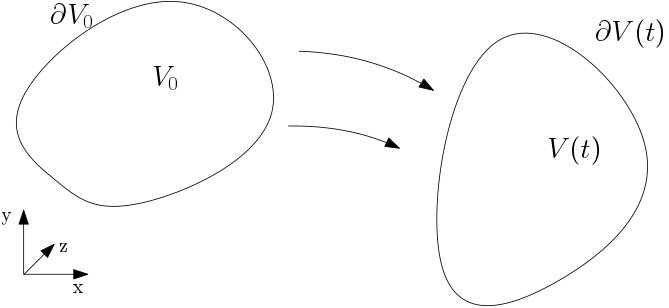
\includegraphics[scale=0.5]{./Fig/unitpotato.png}
      \caption{Unitpotato}
\end{figure}


A \textit{continuum} is defined as a volume $V(t) \subset \mathbb{R}^d \ d \in (2, 3)$ ,  continiously distributed throughout its own volume. The initial shape of the continuum, the \textit{ referenceconfiguration}  $V(t = t_0) = \hat{V}$,  is assumed to be stress free.   When the \textit{continuum} undergoes deformation due to applied internal/external forces , the new configuration $V(t)$ for $t \geq t_0$, can deviate from its \textit{reference configuration}. The new configuration  $V(t) \neq \hat{V}$, is reffered to as the \textit{current configuration}. If the continuum undergoes no deformation, the  \textit{reference} and \textit{current} configuration simply coincide. \\ \\

\section{The lagrangian and eulerian  description of motion}

A fundamental difference between fluid and structure mechanics is the description of motion, the \textit{Lagrangian} and \textit{Eulerian} description. Within structure mechanics, deformation of a continuum due to internal/external forces are of primary interest. When the continuum undergoes deformation, it will deviate from is \textit{reference configuration} $\hat{V}$. To measure the deformation, one must know the relative position of some particle $x(t) \in V(t)$, from its original configuration $\bat{x} \in \hat{V}$. \\

 Let \^{x} be a particle in the reference  $\ha{x} \in \ha{V}$.  Further let x(\^x, t) be the new location of a particle \^x for some time t such that $x \in V(t)$. Assume no two particles $\ha{x}_a, \ha{x}_b \in \ha{V}$ occupy the same location for some time $V(t)$.
Then the transformation $\ha{T}(\ha{x}, t) = x(\ha{x}, t)$ maps a particle \ha{x} from the \textit{reference configuration} $\ha{V}$ to the  \textit{current configuration} $V(t)$
Assuming that the path for some \^{x} is continuous in time, the inverse mapping $\ha{T}^{-1}(x, t) = \ha{x}(x, t)$, maps $x(\ha{x}, t)$ back to its initial location at time $t = t_0$. \\
These mappings lets us track each particle from some \textit{reference configuration} to some deformed state at time t. 
Such a description of tracking each particle $\ha{x} \in \ha{V}$ is often denoted the \textit{Lagrangian Framework} and is a natural choice of describing structure mechanics. 

\begin{figure}[h!]
  \centering
    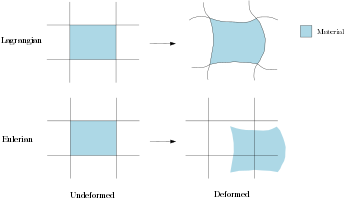
\includegraphics[scale=0.5]{./Fig/lageul.png}
      \caption{Comparison of the Lagrangian and Eulerian description of motion}
\end{figure}


By some particle $/bat{x} \in \bat{V}$, the \textit{deformation} $\bat{u}(\ha{x},t)$ is given by the relation
\begin{align}
\bat{u}(\ha{x},t) = x(\bat{x},t) - \bat{x} = \ha{T}(\bat{x}, t) 
\end{align}

and the \textit{deformation velocity} is given by the time derivative of \textit{deformation} such that
\begin{align}
\bat{v}(\ha{x},t) = d_t x(\bat{x},t) = d_t \bat{u}(\bat{x},t) = \pder{\ha{T}(\ha{x}, t)}{t} 
\end{align}

When tracking each particle as it moves, the \textit{material} and \textit{spatial} points coincide

Considering a flow of fluid particles in a river, a \textit{Lagrangian} description of the particles would be tidious as the number of particles entring and leaving the domain quickly rise to a immense number. 
Instead consider defining a view-point $V$ fixed in time, and monitor every fluid particle passing the coordinate $x \in V(t)$ as time elapses. Such a description is defined as the \textit{Eulerian framework.} 
Therefore the Eulerian formulation is natural for describing fluid dynamics. \\
We can describe the particles occupying the \textit{current configuration} $V(t)$ for some time $t \geq t_0$ 
\begin{align*}
x = \ha{x} + \hat{u}(\ha{x}, t)	
\end{align*}
Since our domain is fixed we can define the deformation for a particle 
occupying position $x = x(\ha{x},t)$ as
\begin{align*}
\textbf{u}(x, t) = \hat{u}(\ha{x}, t) = x - \ha{x}	\\
\end{align*}
and its velocity
\begin{align*}
\textbf{v}(x,t) = \partial_t u(x,t) = \partial_t \hat{u}(\ha{x},t) = \hat{v}(\ha{x},t)
\end{align*}

It is important to mention that the we are not interested in which particle is occupying a certain point in our domain, but only its properties. As such the \textit{material} and \textit{spatial} points doesn't coincide in the \textit{Eulerian formulation}

\subsection{Deformation gradients}
\textit{Deformaion}  is a major property of interest, when a continuum is influenced by external and internal forces.  Deformation, is the 
When studying continuum mechanics we observe continious mediums as they are deformed over time. These deformations results in relative changes of positions due to external and internal forces acting. These relative changes of postition is called \textit{strain}, and is the primary property that causes \textit{stress} within a medium of interest \cite{Richter2016}. We define stress as the internal forces that particles within a continuous material exert on each other. \\

The equations of mechanics can be derived with respect to either a deformed or undeformend configuration of our medium of interest. The choice of refering our equations to the current or reference configuration is indifferent from a theoretical point of view. In practice however this choice can have a severe impact on our strategy of solution methods and physical of modelling.   \cite{Wriggers2006}. We will therefore define the strain measures for both configurations of our medium.  

\begin{defn}
Deformation gradient. 
\begin{align}
\hat{F} = I + \hat{\nabla} \hat{u} 
\end{align} 
\end{defn}

Mind that deformation gradient of $\hat{u}$ is which respect to the reference configuration. 
From the assumption that no two particles $\ha{x}_a, \ha{x}_b \in \ha{V}$ occupy the same location for some time $V(t)$, the presented transformation must be linear. As a consequence from the invertible matrix theorem found in linear algebra, the linear operator \textbf{F} cannot be a singuar.  
We define the  \textit{determinant of the deformation gradient} as \textit{J}, which denotes the local change of volume of our domain. 

\begin{defn}
Determinant of the deformation gradient
\begin{align}
J = det(\hat{F}) = det( I + \hat{\nabla} \hat{u} ) \neq 0
\end{align} 
\end{defn}


By the assumption that the medium can't be selfpenetrated, we must limit  J to be greater than 0 \cite{Wriggers2006}

It is important to note that strain itself is nothing else than the measurement of line segments under deformation. Therefore strain alone is purely an observation, and it is not dependent on the material of interest. However one expects that a material undergoing strain, will give  forces within the material due to neighboring material interacting with one another. Therefore one derive materialspecific models to describe how a certain material will react to a certain amount of strain.\\
These strain measures are used to define models for \textit{stress}, which is responsible for the deformation in materials (cite holzapfel). The dimention of stress is force per unit area.

\newpage
\subsection{The solid problem}



The governing equations for the solid mechanics are given by the blalance law,
\begin{equat}
\textit{Solid momentum}
\begin{align}
\rho_s \pder{\mathbf{v}_s}{t} = \nabla \cdot \bat{T} + \rho_s \mathbf{f}_s
\hspace{4mm} \text{in} \hspace{2mm} \hat{\Omega}_s
\end{align}
\end{equat}
defined in a Lagrangian coordinate system, with respect to an initial reference configuration $\hat{\Omega}_s$. The structure configuration is given by the displacement $\bat{u}_s$, with the relation
 $\pder{\bat{v}}{t} = \bat{u}_s$ to the solid velocity. The density of the structure is given by $\rho_s$, and $\bat{f}_s$ express any exterior body forces acting. The tensor $\bat{T}$ denotes the first Piola-Kirchhoff stress tensor, with the relation $\bat{T}  = \bat{J} \sigma_s \bat{F}^{-T}$ to the cauchy stress tensor. By definition the cauchy stress tensor is symmetric, however the first Piola-Kirchhoff tensor does not exhibit this property. As constitute equations often assumes this behaviour of symmetry, the second Piola-Kirchhoff tensor $\bat{S}_s$ is convenient as it is symmetric.  It is given by the relation to the firt Piola-Kirchhoff stress tensor by, 
 
 \begin{align*}
 \bat{S}_s = \bat{F}^{-T} \bat{T} = \hat{J} \bat{F}^{-1} \sigma_s \bat{F}^{-T}
 \end{align*}
 
According to the material of interest, several material models exist to model the induced stress given by material deformation. Most famous is Hooke's law, describing a linear relation between strain and stress, limited to a small-deformation regime. As we may no longer be in the range of small-deformation approximation were a linear-elastic material can be used, a consitent way to describe large deformations is needed. As such, for describing large deformation it is widley common to use a stress-strain relation based of the introduced Green Lagrangian strain tensor $\bat{E}$ and the second Piola-Kirchhoff stress tensor $\bat{S}$ \cite{Razzaq2010}. Therefore the material is assumed to follow a hyperelastic model, specifically the Vernant-Kirchhoff(STVK) model. Though STVK can handle large deformations, it is limited of the calculation of large strain \cite{Razzaq2010}. However since the deformations considered in this thesis are small, it will remain our primary choice of strain-stress relation.  STVK describes materials of compressible nature,  but is should be mentioned that for large deformation models describing incompressible materials can be considered. Specially the Incompressible Neo-Hooke (INH) model is considered in several publications (see \cite{Wick2013}, \cite{Richter2010c}), sharing the same hyperelastic properties as the STVK model. As both models handles large deformations, the INH is superior compared to STVK in the sense that it is valid for large strains aswell \cite{Razzaq2010}. \newpage
The STVK is one of the simplest hyperelastic model, as it only extend the famous Hooke's law into a non-linear regime by,

\begin{align*}
\sigma_s = \frac{1}{\hat{J}} \bat{F}(\lambda_s(Tr(\bat{E}) I + 2 \mu \bat{E})\bat{F}^{-T} \hspace{4mm}
\bat{S}_s = \lambda_s(Tr(\bat{E}) I + 2 \mu \bat{E} \\
\bat{E} = \frac{1}{2}(\bat{C} - I ) \hspace{4mm} \bat{C} = \bat{F}\bat{F}^{-T}
\end{align*} 
 where $\bat{C}$ is the right Cauchy-Green strain tensor mention in the last subchapter. 
  
 The solid is often characterized by the Possion ratio and Young modulus. Lamè coefficients  $\lambda_s$ and $\mu_s$ are then given by the relation.

\begin{align*}
&E_y = \frac{ \mu_s ( \lambda_s + 2 \mu_s) }{ ( \lambda_s + \mu_s ) } 
\hspace{5mm} \nu_s = \frac{\lambda_s}{2(\lambda_s + \mu_s)} \\
&\lambda_s = \frac{\nu E_y}{(1 + \nu_s)(1 - 2\nu_s)} \hspace{4mm} \mu_s = \frac{E_y}{2(1 + \nu_s)} 
\end{align*}

Since the solid deformation is a quantity of interest a kinematic condition must be defined for the system of the form
\begin{align}
\pder{\mathbf{v}_s}{t} = \mathbf{u_s} \hspace{4mm} \text{in} \hspace{2mm} \Omega_s
\end{align} 
One might ask the motivation of such an approach as the Lagrangian system could let us define the problem 
\begin{align}
\rho_s \ppder{\mathbf{u}_s}{t} = \nabla \cdot \mathbf{T} + \rho_s \mathbf{f}_s
\hspace{4mm} \text{in} \hspace{2mm} \Omega_s
\end{align}
directly solving for the main quantity of interest namely deformation. However solving for $\mathbf{v}_s$ is more convenient, as it lets us handle constraints for the fluid-structure interaction problem easier. As for the fluid problem we define Dirichlet and Neumann boundary conditions on the form

\begin{align*}
\mathbf{v}_s = \mathbf{v}_s^D 
\hspace{4mm} \text{on} \hspace{2mm} \Gamma_s^D \subset \partial \Omega_s  \\
\sigma_s \cdot \mathbf{n} = \mathbf{g}  
\hspace{4mm} \text{on} \hspace{2mm} \Gamma_s^N \subset \partial \Omega_s 
\end{align*}


\section{The Fluid problem}
We will throughout this thesis consider in-compressible fluids described by Navier-Stokes equations. We define the fluid density as $\rho_f$ and fluid viscosity $\nu_f$ to be constant in time. Our phsyical unknowns
fluid velocity $v_f$ and pressure $p_f$ both live in the time-dependent fluid domain  $\hat{\Omega}_f(t)$, with an eulerian configuration. Together with the equations of momentum and continuum, the Navier-Stokes equation is defined as,

\begin{equat}
\textit{Navier-Stokes equation}
\begin{align}
&\rho \pder{\mathbf{v}_f}{t} + \rho \mathbf{v}_f \cdot \nabla \mathbf{v}_f =
\nabla \cdot \sigma + \rho \mathbf{f}_f \hspace{4mm} \text{in} \hspace{2mm} \Omega_f \\
&\nabla \cdot \mathbf{v}_f = 0 \hspace{4mm} \text{in} \hspace{2mm} \Omega_f 
\end{align} 
\end{equat}
where $\mathbf{f}_s$ is some body force. 
Assuming a newtonian fluid the \textit{Cauchy stress sensor} $\sigma$ takes the form \newline $\sigma = -p_f I + \mu_f (\nabla \mathbf{v}_f + (\nabla \mathbf{v}_f)^T$.

Additional appropriate boundary conditions are supplemented to the equation for a given problem. The first type of of boundary conditions are Dirichlet boundary conditions, 
\begin{align}
\mathbf{v}_f = \mathbf{v}_f^D 
\hspace{4mm} \text{on} \hspace{2mm} \Gamma_f^D \subset \partial \Omega_f 
\end{align}
The second type of boundary condition are Neumann boundary conditions
\begin{align}
\sigma_f \cdot \mathbf{n} = \mathbf{g} 
\hspace{4mm} \text{on} \hspace{2mm} \Gamma_f^N \subset \partial \Omega_f 
\end{align}

\section{Sumup}



. serving as a foundation for the  computational fluid-structure interaction problem presented in the next chapter. 